\documentclass[notitlepage,aps,prd,nofootinbib]{revtex4-1}

\usepackage{subfig}
%\usepackage[colorinlistoftodos]{todonotes}
\usepackage{float}

%\usepackage[protrusion=true,expansion=true]{microtype}
\usepackage{amsmath}
\usepackage{amssymb}
\usepackage{bbm}
\usepackage{ulem}
%\usepackage{feynmp-auto}
%\usepackage{slashed}
%\usepackage[absolute,overlay]{textpos}
\usepackage[usenames, dvipsnames]{color}
\usepackage{graphicx}
\usepackage{listings}
\usepackage{epsfig}
\usepackage{hyperref}
%\usepackage{tikz}
\usepackage{enumerate}
%\usepackage{fixltx2e} % buggy
\usepackage[compatibility=false]{caption}
%\usepackage{subcaption} % doesn't work with subfigure
\usepackage{pdfpages}
%\usepackage{setspace}
\usepackage{verbatim}

% Turn off meaningless float warnings
\usepackage{silence}
\WarningFilter{revtex4-1}{Repair the float}

\DeclareRobustCommand{\orderof}{\ensuremath{\mathcal{O}}}

\definecolor{dukeblue}{RGB}{0,0,156}
\definecolor{dukedarkblue}{RGB}{0,26,87}
\definecolor{dukeblack}{RGB}{79,79,79}
\definecolor{dukegray}{RGB}{79,79,79}
\definecolor{dukesecbrown}{RGB}{217,200,158}
\definecolor{dukesecblue}{RGB}{127,169,174}

%\renewcommand*{\thefootnote}{\fnsymbol{footnote}}

%%%%%%%%%%%%%%%%%%%%%%%%%%%%%%%%%%%%%%%%%%%%%%%%%%%%%%%%%%%%%%%%%%%%%%%%%%%%%%%%%%%%%
\hypersetup{
    breaklinks,
    baseurl       = http://,
    pdfborder     = 0 0 0,
    pdfpagemode   = UseNone,% do not show thumbnails or bookmarks on opening
    pdfstartpage  = 1,
    bookmarksopen = true,
    bookmarksdepth= 2,% to show sections and subsections
% revtex needs author and title declared after \begin{document}, so have to hard code them...
%    pdfauthor     = {\@author},
%    pdftitle      = {\@title},
    pdfauthor     = {Matthew Epland},
    pdftitle      = {Phys 566 HW4},
    pdfsubject    = {},
    pdfkeywords   = {}}


% Code import settings
%%%%%%%%%%%%%%%%%%%%%%%%%%%%%%%%%%%%%%%%%%%%%%%%%%%%%%%%%%%%%%%%%%%%%%%%%%%%%%%%%%%%%
\definecolor{mygreen}{rgb}{0,0.6,0}
\definecolor{mygray}{rgb}{0.5,0.5,0.5}
\definecolor{mymauve}{rgb}{0.58,0,0.82}

%\lstset{ %
\lstdefinestyle{python}{ %
  backgroundcolor=\color{white},   % choose the background color; you must add \usepackage{color} or \usepackage{xcolor}
  basicstyle=\scriptsize,          % the size of the fonts that are used for the code
  breakatwhitespace=false,         % sets if automatic breaks should only happen at whitespace
  breaklines=true,                 % sets automatic line breaking
  captionpos=b,                    % sets the caption-position to bottom
  commentstyle=\color{mygreen},    % comment style
  deletekeywords={...},            % if you want to delete keywords from the given language
  escapeinside={\%*}{*)},          % if you want to add LaTeX within your code
  extendedchars=true,              % lets you use non-ASCII characters; for 8-bits encodings only, does not work with UTF-8
  frame=single,	                   % adds a frame around the code
  keepspaces=true,                 % keeps spaces in text, useful for keeping indentation of code (possibly needs columns=flexible)
  keywordstyle=\color{blue},       % keyword style
  language=Python,                 % the language of the code
  otherkeywords={*,...},           % if you want to add more keywords to the set
  numbers=left,                    % where to put the line-numbers; possible values are (none, left, right)
  numbersep=5pt,                   % how far the line-numbers are from the code
  numberstyle=\tiny\color{mygray}, % the style that is used for the line-numbers
  rulecolor=\color{black},         % if not set, the frame-color may be changed on line-breaks within not-black text (e.g. comments (green here))
  showspaces=false,                % show spaces everywhere adding particular underscores; it overrides 'showstringspaces'
  showstringspaces=false,          % underline spaces within strings only
  showtabs=false,                  % show tabs within strings adding particular underscores
  stepnumber=5,                    % the step between two line-numbers. If it's 1, each line will be numbered
  stringstyle=\color{mymauve},     % string literal style
  tabsize=2,	                   % sets default tabsize to 2 spaces
%  title=\lstname                   % show the filename of files included with \lstinputlisting; also try caption instead of title
  title={\protect\filename@parse{\lstname}\protect\filename@base.\filename@ext},
  firstnumber=0,
%  linewidth=0.95\textwidth
  xleftmargin=0.01\textwidth,
  xrightmargin=0.01\textwidth
}

\lstdefinestyle{output}{ %
  backgroundcolor=\color{white},   % choose the background color; you must add \usepackage{color} or \usepackage{xcolor}
  basicstyle=\scriptsize,          % the size of the fonts that are used for the code
  breakatwhitespace=false,         % sets if automatic breaks should only happen at whitespace
  breaklines=true,                 % sets automatic line breaking
  captionpos=b,                    % sets the caption-position to bottom
  escapeinside={\%*}{*)},          % if you want to add LaTeX within your code
  frame=single,	                   % adds a frame around the code
  keepspaces=true,                 % keeps spaces in text, useful for keeping indentation of code (possibly needs columns=flexible)
  numbers=left,                    % where to put the line-numbers; possible values are (none, left, right)
  numbersep=5pt,                   % how far the line-numbers are from the code
  numberstyle=\tiny\color{mygray}, % the style that is used for the line-numbers
  rulecolor=\color{black},         % if not set, the frame-color may be changed on line-breaks within not-black text (e.g. comments (green here))
  stepnumber=5,                    % the step between two line-numbers. If it's 1, each line will be numbered
  tabsize=2,	                   % sets default tabsize to 2 spaces
%  title=\lstname                   % show the filename of files included with \lstinputlisting; also try caption instead of title
  title={\protect\filename@parse{\lstname}\protect\filename@base.\filename@ext},
  firstnumber=0,
%  linewidth=0.95\textwidth
  xleftmargin=0.01\textwidth,
  xrightmargin=0.01\textwidth
}

\newcommand{\degree}{\ensuremath{^{\circ}}}

% Select between raw and saved plots here
\graphicspath{{../code/output/plots_for_paper/}} % raw plots
%\graphicspath{{./output/}} % saved plots

%%%%%%%%%%%%%%%%%%%%%%%%%%%%%%%%%%%%%%%%%%%%%%%%%%%%%%%%%%%%%%%%%%%%%%%%%%%%%%%%%%%%%
\begin{document}

\title{PHYS 566 HW4}
\author{Matthew Epland}
\affiliation{Department of Physics, Duke University, Durham, NC 27707, USA}

\date{\today}

\begin{abstract}
In this assignment the behavior of a dampened, driven simple pendulum was investigated numerically via the $\orderof\big(\left(\Delta t\right)^2\big)$ Euler--Cromer and $\orderof\big(\left(\Delta t\right)^4\big)$ Rung--Kutta methods. The pendulum's resonance curves, nonlinear behavior, and chaotic properties were studied for a variety of driving frequencies, amplitudes, and initial conditions.
\end{abstract}\maketitle


\section{Introduction}
\label{sec:intro}
Damped, driven pendulums are a rich second order system for study, exhibiting many interesting behaviors such as resonance, nonlinear equations, and chaos. Furthermore they are a good system to model computationally as analytical solutions can be derived, in the limit of the linear, small angle approximation. In this assignment a damped, driven simple pendulum was simulated with the Euler--Cromer and Rung--Kutta methods. By varying parameters of the system resonance, nonlinear effects and chaos were studied in turn, as well as the differences between the two simulation methods themselves.

\section{Theory}
\label{sec:theory}
The equation of motion of a damped, driven pendulum (\ref{eq:diff_eq}) for small angles\footnote{Where $\sin\left(\theta\right) \approx \theta + \orderof\left(\theta^2\right)$} is a second order linear equation. As written all of the constants are positive real numbers. It is helpful to rewrite (\ref{eq:diff_eq}) as (\ref{eq:diff_eq2}) where $\omega_{0}^2 = g/l$ and $F\left(t\right)$ is the external driving force.

\begin{equation} \label{eq:diff_eq}
\frac{d^2 \theta}{d t^2} = -\frac{g}{l}\theta - 2\gamma\frac{d \theta}{d t} + \alpha_{D}\sin\left(\Omega_{D} t\right)
\end{equation}

\begin{equation} \label{eq:diff_eq2} 
\begin{gathered}
\ddot{\theta} + 2\gamma \dot{\theta} + \omega_{0}^2 \theta = F\left(t\right) \\
F\left(t\right) = \alpha_{D} \sin\left(\Omega_{D} t\right)
\end{gathered}
\end{equation}

The solution to (\ref{eq:diff_eq2}) can be broken into two parts, the solution of the associated homogeneous equation where $F\left(t\right) = 0$ and any particular solution of (\ref{eq:diff_eq2}). To begin with we will solve the homogeneous equation by assuming a solution of the form $\theta\left(t\right) \sim e^{r t}$, which is indeed a solution provided that $r$ is a root of the characteristic equation (\ref{eq:characteristic_eq}). Using the quadratic formula we find the two roots to be $r_{\pm}$ (\ref{eq:r_pm}), thereby specifying the homogeneous solution\footnote{If $\gamma = \omega_{0}$, and therefore $r_{+} = r_{-}$, we need to include a multiplicative factor of $t$ on one of the solutions so that they are linearly independent.} (\ref{eq:homogeneous_soln}). 

\begin{gather}
r^2 + 2 \gamma r + \omega_{0}^2 = 0 \label{eq:characteristic_eq} \\
r_{\pm} = -\gamma \pm \sqrt{\gamma^2 - \omega_{0}^2} \label{eq:r_pm}
\end{gather}

\begin{equation} \label{eq:homogeneous_soln}
\theta\left(t\right)_{\text{Homogeneous}} =
\begin{cases}
A e^{r_{+} t} + B e^{r_{-} t} & \text{if } \gamma \neq \omega_{0} \\
\left(A + B t\right) e^{-\gamma t} & \text{if } \gamma = \omega_{0}
\end{cases}
\end{equation}

It is easy to see from (\ref{eq:r_pm}) that $\operatorname{Re}\left(r_{\pm}\right) < 0$ for all $\gamma$ and $\omega_{0}$, therefore the homogeneous solution (\ref{eq:homogeneous_soln}) always decays away to nothing; it is a transient solution\footnote{The homogeneous solutions importance in this case lies in it's ability to match the initial conditions of the pendulum, regardless of what the driving force is doing. For our pendulum the initial conditions are $\theta\left(t=0\right)=\theta_{0},~\omega\left(t=0\right)=0$}. As we are primary interested in the steady state behavior of the pendulum in this assignment we therefore need only be concerned with the particular solution from here on out.

We can find a particular, or steady state, solution (\ref{eq:particular_soln}) that works by trial and error. Plugging (\ref{eq:particular_soln}) into (\ref{eq:diff_eq2}) with $F\left(t\right) = \alpha_{D} \sin\left(\Omega_{D} t\right)$ results in (\ref{eq:particular_work}).

\begin{equation} \label{eq:particular_soln}
\theta\left(t\right)_{\text{Particular}} = \theta_{P} \sin\left(\Omega_{D} t - \phi\right)
\end{equation}

\begin{equation} \label{eq:particular_work}
\frac{\alpha_{D}}{\theta_{P}} \sin\left(\Omega_{D} t\right) = \left(\omega_{0}^2 - \Omega_{D}^2\right) \sin\left(\Omega_{D} t - \phi\right) + 2 \gamma \Omega_{D} \cos\left(\Omega_{D} t - \phi\right)
\end{equation}

While (\ref{eq:particular_work}) may look messy, we can extract the steady state amplitude $\theta_{P}\left(\Omega_{D}\right)$ and phase $\phi\left(\Omega_{D}\right)$ by making use of the trigonometric identity (\ref{eq:trig_identity}) with $\alpha = \Omega_{D} t - \phi$ and $\beta = \phi$. Rearranging (\ref{eq:particular_work}) into (\ref{eq:particular_work2}), we can identify (\ref{eq:particular_work3}) term by term.

\begin{equation} \label{eq:trig_identity}
\sin\left(\alpha + \beta\right) = \sin\left(\alpha\right) \cos\left(\beta\right) + \cos\left(\alpha\right) \sin\left(\beta\right)
\end{equation}

\begin{equation} \label{eq:particular_work2}
\sin\left(\alpha + \beta\right) = \sin\left(\alpha\right) \bigg(\frac{\theta_{P}}{\alpha_{D}} \left(\omega_{0}^2 - \Omega_{D}^2\right)\bigg) + \cos\left(\alpha\right) \bigg(\frac{2 \gamma \Omega_{D} \theta_{P}}{\alpha_{D}}\bigg)
\end{equation}

\begin{align}
\label{eq:particular_work3}
\cos\left(\phi\right) &= \frac{\theta_{P}}{\alpha_{D}} \left(\omega_{0}^2 - \Omega_{D}^2\right)
&
\sin\left(\phi\right) &=  \frac{2 \gamma \Omega_{D} \theta_{P}}{\alpha_{D}}
\end{align}

Now that $\sin\left(\phi\right)$ and $\cos\left(\phi\right)$ are known, $\theta_{P}\left(\Omega_{D}\right)$ and $\phi\left(\Omega_{D}\right)$ (\ref{eq:thetaP} and \ref{eq:phi}) can be found from the sum of their squares and their ratio, respectively.

\begin{equation} \label{eq:thetaP}
\theta_{P}\left(\Omega_{D}\right) = \frac{\alpha_{D}}{\sqrt{ \left(\omega_{0}^2 - \Omega_{D}^2\right)^2 + 4 \gamma^2 \Omega_{D}^2 }}
\end{equation}

\begin{equation} \label{eq:phi}
\phi\left(\Omega_{D}\right) = \arctan\left(\frac{2 \gamma \Omega_{D}}{\omega_{0}^2 - \Omega_{D}^2}\right)
\end{equation}

\subsection{Resonance}
\label{subsec:resonance}
As our pendulum is a driven oscillator we can expect it to exhibit resonant behavior at some driving frequency, $\Omega_{\text{Res}}$. To find $\Omega_{\text{Res}}$ analytically we can employ the usual maximization method\footnote{Of course this result could be a minimum of $\theta_{P}\left(\Omega_{D}\right)$, but in this case it is indeed a maximum as later figures show.} of solving for where the first derivative is zero (\ref{eq:resonance_derivative}).

\begin{equation} \label{eq:resonance_derivative}
0 = \left.\frac{d \theta_{P}}{d \Omega_{D}}\right|_{\Omega_{D} = \Omega_{\text{Res}}}
= -\frac{\alpha_{D}}{2} \bigg( \left(\omega_{0}^2 - \Omega_{\text{Res}}^2\right)^2 + 4 \gamma^2 \Omega_{\text{Res}}^2 \bigg)^{-3/2}
\bigg(- 4 \left(\omega_{0}^2 - \Omega_{\text{Res}}^2\right) \Omega_{\text{Res}} + 8 \gamma^2 \Omega_{\text{Res}} \bigg)
\end{equation}

\begin{equation} \label{eq:omegaD_resonance}
\Omega_{\text{Res}} = \sqrt{ \omega_{0}^2 - 2 \gamma^2} 
\end{equation}

Lastly, note that $\Omega_{\text{Res}}$ of (\ref{eq:omegaD_resonance}) solves (\ref{eq:resonance_derivative}) when $\omega_{0} \neq \gamma$. If $\omega_{0} \approx \gamma$ the $(\cdots)^{-3/2}$ term diverges and we would need to set $\gamma = \omega_{0}$ at the beginning of the problem and redo the derivation. Fortunately for the parameters used in this assignment we have $\omega_{0} = 1.0~s^{-1} \neq \gamma = 0.25~s^{-1} \rightarrow \Omega_{\text{Res}} =$ 0.93541 [rad/s], so this is not an issue.

\subsection{Euler--Cromer}
\label{subsec:eulercromer}
In the past we have used the Euler method solve differential equations time step to time step. The advantage of using the Euler method is its simplicity, however its solutions usually do not conserve energy but increase in total energy over time. We can remedy this by switching to the Euler--Cromer method, also known as the semi-implicit Euler method\footnote{The name semi-implicit comes from the fact that $n+1$ data in the form of $\omega_{n+1}$ is being used to compute $\theta_{n+1}$. Also note that like the unmodified Euler method, the Euler--Cromer method is still only a $\orderof\big(\left(\Delta t\right)^2\big)$ method.}, by modifying the Euler method to use $\omega_{n+1}$ instead of $\omega_{n}$ when computing $\theta_{n+1}$, see (\ref{eq:euler_chromer1}, \ref{eq:euler_chromer2}).

\begin{align}
\frac{d \theta}{d t} &= f\left(t, \theta;~\omega\right) &
\frac{d \omega}{d t} &= \frac{d^2 \theta}{d t^2} = g\left(t, \omega;~\theta\right) \label{eq:euler_chromer1} \\
\theta_{n+1} &= \theta_{n} + f\left(t_{n}, \theta_{n};~\underline{\omega_{n+1}}\right) \Delta t & 
\omega_{n+1} &= \omega_{n} + g\left(t_{n}, \omega_{n};~\theta_{n}\right) \Delta t \label{eq:euler_chromer2}
\end{align}

\begin{equation} \label{eq:tn} 
t_{n} = t_{0} + n \Delta t = n \Delta t
\end{equation}

For our pendulum we have:
\begin{align} \label{eq:f_g_applied}
f\left(t, \theta;~\omega\right) &=  \omega &
g\left(t, \omega;~\theta\right) &= -\omega_{0}^2 \theta - 2\gamma \omega + \alpha_{D}\sin\left(\Omega_{D} t\right)
\end{align}

\subsection{Runge--Kutta}
\label{subsec:runge_kutta}
The Euler and Euler--Cromer methods work by sampling the differential equation once at the beginning of each time step interval, which when worked out gives them a final error of $\orderof\big(\left(\Delta t\right)^2\big)$. As such, an easy way to improve on the Euler method is to sample the differential equation more than once per time step. The family of numerical solutions of this type are called Runge--Kutta methods, of which the Euler method is the simplest member. For this assignment in addition to the Euler--Cromer method we will be using \textit{The} Runge--Kutta method, or RK4, which samples the differential equation four times per time step. The four samples are used in a weighted average in place of $f\left(t\right)$ and $g\left(t\right)$ in the Euler method, compare (\ref{eq:euler_chromer1}, \ref{eq:euler_chromer2}) to (\ref{eq:RK4_1}, \ref{eq:RK4_2}). By averaging over four samples per time step the RK4 method decreases the error to $\orderof\big(\left(\Delta t\right)^4\big)$, quite a nice improvement for relatively little effort.\footnote{Naturally we could also alter the RK4 method to be an implicit method like the Euler--Cromer method, but will not in this assignment to avoid further complexity.} For our pendulum $f\left(t\right)$ and $g\left(t\right)$ remain the same as before (\ref{eq:f_g_applied}).

\begin{align}
\theta_{n+1} &= \theta_{n} + \frac{1}{6}\left(k_{1} + 2k_{2} +2k_{3} +k_{4}\right)\Delta t &
\omega_{n+1} &= \omega_{n} + \frac{1}{6}\left(l_{1} + 2l_{2} +2l_{3} +l_{4}\right)\Delta t \label{eq:RK4_1} \\
\begin{split}
k_{1} &= f\left(t_{n}, \theta_{n};~\omega_{n}\right) \\
k_{2} &= f\left(t_{n} +\Delta t/2, \theta_{n}+k_{1}\Delta t/2;~\omega_{n}+l_{1}\Delta t/2\right) \\
k_{3} &= f\left(t_{n} +\Delta t/2, \theta_{n}+k_{2}\Delta t/2;~\omega_{n}+l_{2}\Delta t/2\right) \\
k_{4} &= f\left(t_{n} +\Delta t, \theta_{n}+k_{3}\Delta t;~\omega_{n}+l_{3}\Delta t\right)
\end{split} &
\begin{split}
l_{1} &= g\left(t_{n}, \omega_{n};~\theta_{n}\right) \\
l_{2} &= g\left(t_{n} +\Delta t/2, \omega_{n}+l_{1}\Delta t/2;~\theta_{n}+k_{1}\Delta t/2\right) \\
l_{3} &= g\left(t_{n} +\Delta t/2, \omega_{n}+l_{2}\Delta t/2;~\theta_{n}+k_{2}\Delta t/2\right) \\
l_{4} &= g\left(t_{n} +\Delta t, \omega_{n}+l_{3}\Delta t;~\theta_{n}+k_{3}\Delta t\right)
\end{split} \label{eq:RK4_2}
\end{align}





\clearpage
\section{Results}
\label{sec:results}

\subsection{Parts B and C: Vary Simulation Methods}
\label{subsec:vary_sim_methods}
We will begin by comparing the results of the two simulation methods, Euler--Cromer and RK4, by looking at plots of $\theta\left(t\right)$, $\omega\left(t\right)$, and energy versus time. As you can see in Figures~\ref{fig:theta_vary_sim_method},~\ref{fig:omega_vary_sim_method},~\ref{fig:energy_Euler-Cromer}, and~\ref{fig:energy_RK4}, both methods produced virtually identical results for this pendulum. For the energy plots note that we do not expect total energy to be conserved, even at steady state, because $F_{\text{Driving}}$ and $F_{\text{Dampening}}$ are external forces that continually doing work on the system. If we turn them off, $\alpha_{D} = 0.0$, $\gamma = 0.0$, we do have energy conservation, see Section~\ref{subsec:E_conservation}.

\begin{figure}[!htbc]
  \centering
  \includegraphics[width=.6\textwidth]{part_b/compare_runs_vary_sim_method/theta_vary_sim_method.pdf}
	{\par\nobreak\rule[9pt]{35em}{0.5pt}\vspace{-5mm}}
	\caption{$\theta\left(t\right)$ for the Euler--Cromer and RK4 methods.}
	\label{fig:theta_vary_sim_method}
\end{figure}

\begin{figure}[!htbc]
  \centering
  \includegraphics[width=.6\textwidth]{part_b/compare_runs_vary_sim_method/omega_vary_sim_method.pdf}
	{\par\nobreak\rule[9pt]{35em}{0.5pt}\vspace{-5mm}}
	\caption{$\omega\left(t\right)$ for the Euler--Cromer and RK4 methods.}
	\label{fig:omega_vary_sim_method}
\end{figure}

\begin{figure}[!htbc]
  \centering
  \includegraphics[width=.8\textwidth]{part_c/energy/energy_Euler-Cromer.pdf}
	{\par\nobreak\rule[9pt]{35em}{0.5pt}\vspace{-5mm}}
	\caption{Kinetic, potential and total energy when using the Euler--Cromer method.}
	\label{fig:energy_Euler-Cromer}
\end{figure}

\begin{figure}[!htbc]
  \centering
  \includegraphics[width=.8\textwidth]{part_c/energy/energy_RK4.pdf}
	{\par\nobreak\rule[9pt]{35em}{0.5pt}\vspace{-5mm}}
	\caption{Kinetic, potential and total energy when using the RK4 method.}
	\label{fig:energy_RK4}
\end{figure}

\clearpage
\subsection{Part B: Resonance}
\label{subsec:resonance_results}
For the rest of the results we will use the RK4 method to simulate the pendulum. By fitting the steady state $\theta\left(t\right)$ curve with a sinusoid we are able to extract $\theta_{P}\left(\Omega_{D}\right)$ and $\phi\left(\Omega_{D}\right)$ for many different value of $\Omega_{D}$ about $\Omega_{\text{Res}}$, see Figures~\ref{fig:res_sweep_thetaP_1} and~\ref{fig:res_sweep_phi_1}. The code was written to automatically perform the fit after waiting a preset number of driving force periods to ensure the steady state had been reached. Supporting plots were made for each $\Omega_{D}$ tested to confirm the fit was good and only included the steady state wave, see Figures~\ref{fig:res_run_omegaD_over_omega_res_theory_1} and~\ref{fig:res_run_omegaD_over_omega_res_theory_fit_region_1} for one example at $\Omega_{D} = 1.6688$ [rad/s].

The $\theta_{P}\left(\Omega_{D}\right)$ resonance peak itself was fit twice, to a Gaussian with an offset and to the form of the analytical curve derived earlier (\ref{eq:thetaP}). As you can see in Figure~\ref{fig:res_sweep_thetaP_1} the analytical ``Spectrum Fit'' matched the simulation data and the theory curve extremely well, all the fit parameters match to five decimal places. This validates our analytical derivation in Section~\ref{sec:theory} or our code, depending on which you initially trust more. On the other hand, the Gaussian fit was very poor; which is not surprising considering the analytical curve is not symmetric. The chief reason for fitting with a Gaussian is the assignment asked us to compare the Full Width at Half Maximum\footnote{With the offset included, the FWHM = $2\sigma\sqrt{-2\ln{\left(2^{-1} (1-(\text{offset}/\text{amplitude}))\right)}}$, which reduces to the usual FWHM if offset = 0.} to $\gamma$. The Gaussian fit's FWHM was $\approx 4\gamma$ suggesting that $\gamma^2$ sets the width of the resonance peak, though this is better seen analytically in (\ref{eq:thetaP}) as well as in Section~\ref{subsec:mathematica_plot}.

\begin{figure}[!htbc]
  \centering
  \includegraphics[width=.95\textwidth]{part_b/res_sweep_rk4_linear/res_sweep_thetaP.pdf}
	{\par\nobreak\rule[9pt]{35em}{0.5pt}\vspace{-5mm}}
	\caption{$\theta_{P}\left(\Omega_{D}\right)$ resonance curve and fits.}
	\label{fig:res_sweep_thetaP_1}
\end{figure}

\clearpage
The $\phi\left(\Omega_{D}\right)$ resonance peak was fit with the analytical curve (\ref{eq:phi}). Again there was very good agreement between the simulation data, the analytical fit curve, and the analytical theory.

\begin{figure}[!htbc]
  \centering
  \includegraphics[width=.95\textwidth]{part_b/res_sweep_rk4_linear/res_sweep_phi.pdf}
	{\par\nobreak\rule[9pt]{35em}{0.5pt}\vspace{-5mm}}
	\caption{$\phi\left(\Omega_{D}\right)$ resonance curve and fit.}
	\label{fig:res_sweep_phi_1}
\end{figure}

\clearpage
\begin{figure}[!htbc]
  \centering
  \includegraphics[width=.7\textwidth]{{part_b/res_sweep_rk4_linear/res_runs/res_run_omegaD_over_omega_res_theory_1.78}.pdf}
	{\par\nobreak\rule[9pt]{35em}{0.5pt}\vspace{-5mm}}
	\caption{$\theta\left(t\right)$ at $\Omega_{D} = 1.6688$ [rad/s], full view. Note how the fit is performed on data well into the steady state region.}
	\label{fig:res_run_omegaD_over_omega_res_theory_1}
\end{figure}

\begin{figure}[!htbc]
  \centering
  \includegraphics[width=.7\textwidth]{{part_b/res_sweep_rk4_linear/res_runs/res_run_omegaD_over_omega_res_theory_1.78_fit_region}.pdf}
	{\par\nobreak\rule[9pt]{35em}{0.5pt}\vspace{-5mm}}
	\caption{$\theta\left(t\right)$ at $\Omega_{D} = 1.6688$ [rad/s], fit region. The sinusoidal fit typically matched the theory predictions to all the shown decimal places. This $\Omega_{D}$ plot was chosen to be included in particular to illustrate that the data was really being fit -- you can see a difference in the last decimal place of the $\phi$ values.}
	\label{fig:res_run_omegaD_over_omega_res_theory_fit_region_1}
\end{figure}


\clearpage
\subsection{Part D: Nonlinear Effects}
\label{subsec:nonlinear_effects}
As we are running a numerical simulation there is no problem in abandoning the small angle approximation and having the restoring force go as $-\omega_{0}^2 \sin\left(\theta\right)$. We only need to change $g\left(t, \omega;~\theta\right)$ to (\ref{eq:nonlinear_g}) and the Euler--Cromer and RK4 methods will run as easily as before. This is in sharp contrast to the difficultly of attempting to redo the analytical derivation.

\begin{equation}
\label{eq:nonlinear_g}
g\left(t, \omega;~\theta\right)_{\text{nonlinear}} = -\omega_{0}^2 \sin\left(\theta\right) - 2\gamma \omega + \alpha_{D}\sin\left(\Omega_{D} t\right)
\end{equation}

When the driving force is small, $\alpha_{D} = 0.2$ [rad/s$^2$], the pendulum does not move far from $\theta = 0$. In this case we expect the small angle approximation hold, and indeed there are no real differences between the linear and nonlinear simulations, see Figures~\ref{fig:theta_vary_linearity_low_alphaD} and~\ref{fig:omega_vary_linearity_low_alphaD}. However, when the driving force is increased, $\alpha_{D} = 1.2$ [rad/s$^2$], it drives the pendulum up to higher $\theta$'s, breaking the small angle approximation. In this case significant deviations occur between the linear and nonlinear simulations, see Figures~\ref{fig:theta_vary_linearity_high_alphaD} and~\ref{fig:omega_vary_linearity_high_alphaD}. The nonlinear simulation is the correct method to use here, and really could be used always just to be on the safe side. 

\clearpage
\begin{figure}[!htbc]
  \centering
  \includegraphics[width=.75\textwidth]{part_d/compare_runs_vary_linearity_low_alphaD/theta_vary_linearity_low_alphaD.pdf}
	{\par\nobreak\rule[9pt]{35em}{0.5pt}\vspace{-5mm}}
	\caption{$\theta\left(t\right)$ for the linear and nonlinear restoring force, $\alpha_{D} = 0.2$ [rad/s$^2$].}
	\label{fig:theta_vary_linearity_low_alphaD}
\end{figure}

\begin{figure}[!htbc]
  \centering
  \includegraphics[width=.75\textwidth]{part_d/compare_runs_vary_linearity_low_alphaD/omega_vary_linearity_low_alphaD.pdf}
	{\par\nobreak\rule[9pt]{35em}{0.5pt}\vspace{-5mm}}
	\caption{$\omega\left(t\right)$ for the linear and nonlinear restoring force, $\alpha_{D} = 0.2$ [rad/s$^2$].}
	\label{fig:omega_vary_linearity_low_alphaD}
\end{figure}

\clearpage
\begin{figure}[!htbc]
  \centering
  \includegraphics[width=.75\textwidth]{part_d/compare_runs_vary_linearity_high_alphaD/theta_vary_linearity_high_alphaD.pdf}
	{\par\nobreak\rule[9pt]{35em}{0.5pt}\vspace{-5mm}}
	\caption{$\theta\left(t\right)$ for the linear and nonlinear restoring force, $\alpha_{D} = 1.2$ [rad/s$^2$].}
	\label{fig:theta_vary_linearity_high_alphaD}
\end{figure}

\begin{figure}[!htbc]
  \centering
  \includegraphics[width=.75\textwidth]{part_d/compare_runs_vary_linearity_high_alphaD/omega_vary_linearity_high_alphaD.pdf}
	{\par\nobreak\rule[9pt]{35em}{0.5pt}\vspace{-5mm}}
	\caption{$\omega\left(t\right)$ for the linear and nonlinear restoring force, $\alpha_{D} = 1.2$ [rad/s$^2$].}
	\label{fig:omega_vary_linearity_high_alphaD}
\end{figure}


\clearpage
\subsection{Part E: Chaos and Lyapunov Exponents}
\label{subsec:lyapunov}
When working through the theory of the linear pendulum we showed that the initial conditions only affected the transient solution which decayed away exponentially to leave the steady state sinusoid. As such two different pendulums, or systems, with slightly different initial conditions are expected to converge over time. However if we force the pendulum to behave nonlinearly, by increasing $\alpha_{D}$ or $\theta_{0}$ till the small angle approximation breaks down, we must use $-\omega_{0}^2 \sin\left(\theta\right)$ as the restoring force and can no longer rely on the linear theory. Now if two nonlinear systems are setup with very slightly different initial conditions they may no longer converge, but instead diverge exponentially over time\footnote{Each system is still fully deterministic once the initial conditions are specified. Chaotic system are just extremely sensitive to the initial conditions}. Systems displaying such exponential divergence for small changes in initial conditions are classified as chaotic and can be quantitatively described by a Lyapunov Exponent $\lambda$, defined in (\ref{eq:lyapunov_exp}) where $\left|\Delta\theta\left(t\right)\right|$ is the difference in position\footnote{In general we can look at the difference in phase space, but position is fine here.} between the systems at time $t$ and $\left|\Delta\theta_{0}\right|$ is the difference in initial position.

\begin{equation}
\label{eq:lyapunov_exp}
\big|\Delta\theta\left(t\right)\big| = \big|\Delta\theta_{0}\big|e^{\lambda t}
\end{equation}

While any combination of initial conditions can be altered to produce chaotic behavior, we will only be changing $\theta_{0}$ itself by 0.001 $\leq \Delta\theta_{0} \leq$ 0.005 [rad/s] in our simulation. The resulting $\left|\Delta\theta\left(t\right)\right|$ values are so small we instead plot $\ln\left(\left|\Delta\theta\left(t\right)/\Delta\theta_{0}\right|\right)$ which also helps by linearizing the data. To find $\lambda$ we then fit the linearized plot with (\ref{eq:lyapunov_fit})\footnote{An offset $c$ is included so the fit is not overly constrained, even though $c$ should ideally be 0 as we have already divided by $\Delta\theta_{0}$.} over the region in time where the systems are exponentially diverging.

\begin{equation}
\label{eq:lyapunov_fit}
\ln\Bigg(\bigg|\frac{\Delta\theta\left(t\right)}{\Delta\theta_{0}}\bigg|\Bigg) = c_{\text{Fit}} + \lambda_{\text{Fit}} t
\end{equation}

By repeating the simulation and fit multiple times for small changes in $\Delta\theta_{0}$ we can average the $\lambda_{\text{Fit}}$'s and come up with an estimate of $\lambda$ of the system. Three different driving force amplitudes where considered in turn, $\alpha_{D} =$ 0.2, 0.5, and 1.2 [rad/s$^2$]. The first two where small enough that the system behaved linearly and did not exhibit chaos, indeed the $\lambda_{\text{Fit}}$'s $<$ 0 verified the transient exponential decay, see Figures~\ref{fig:Dtheta_0.2}--\ref{fig:lambda_0.5}.

For $\alpha_{D}$ = 1.2 [rad/s$^2$], previously looked at in Section~\ref{subsec:nonlinear_effects}, the system was again nonlinear and showed chaotic behavior, see Figure~\ref{fig:Dtheta_1.2}. The mean $\lambda_{\text{Fit}}$ was found to be 0.1251 [s$^{-1}$], although the structure in Figure~\ref{fig:lambda_1.2} shows that the mean alone may not adequately describe the situation. For the purposes of this computational assignment we will leave it here, though further work more interested in the particulars of system itself should investigate this issue further.

\clearpage
\begin{figure}[!htbc]
  \centering
  \includegraphics[width=.75\textwidth]{{part_e/lyapunov_ave/ave_of_alphaD_0.2_theta0_0.000_rk4/runs/alphaD_0.2_theta0_0.000_Delta_theta0_0.002000_rk4}.pdf}
	{\par\nobreak\rule[9pt]{35em}{0.5pt}\vspace{-5mm}}
	\caption{$\big|\Delta\theta\left(t\right)\big|$ curve and linear fit, $\alpha_{D} = 0.2$ [rad/s$^2$], nonchaotic regime.}
	\label{fig:Dtheta_0.2}
\end{figure}

\begin{figure}[!htbc]
  \centering
  \includegraphics[width=.75\textwidth]{{part_e/lyapunov_ave/ave_of_alphaD_0.2_theta0_0.000_rk4/ave_of_alphaD_0.2_theta0_0.000_rk4_means_plot}.pdf}
	{\par\nobreak\rule[9pt]{35em}{0.5pt}\vspace{-5mm}}
	\caption{$\lambda_{\text{Fit}}$ curve and mean, $\alpha_{D} = 0.2$ [rad/s$^2$], nonchaotic regime.}
	\label{fig:lambda_0.2}
\end{figure}

\clearpage
\begin{figure}[!htbc]
  \centering
  \includegraphics[width=.75\textwidth]{{part_e/lyapunov_ave/ave_of_alphaD_0.5_theta0_0.000_rk4/runs/alphaD_0.5_theta0_0.000_Delta_theta0_0.002000_rk4}.pdf}
	{\par\nobreak\rule[9pt]{35em}{0.5pt}\vspace{-5mm}}
	\caption{$\big|\Delta\theta\left(t\right)\big|$ curve and linear fit, $\alpha_{D} = 0.5$ [rad/s$^2$], nonchaotic regime.}
	\label{fig:Dtheta_0.5}
\end{figure}

\begin{figure}[!htbc]
  \centering
  \includegraphics[width=.75\textwidth]{{part_e/lyapunov_ave/ave_of_alphaD_0.5_theta0_0.000_rk4/ave_of_alphaD_0.5_theta0_0.000_rk4_means_plot}.pdf}
	{\par\nobreak\rule[9pt]{35em}{0.5pt}\vspace{-5mm}}
	\caption{$\lambda_{\text{Fit}}$ curve and mean, $\alpha_{D} = 0.5$ [rad/s$^2$], nonchaotic regime.}
	\label{fig:lambda_0.5}
\end{figure}

\clearpage
\begin{figure}[!htbc]
  \centering
  \includegraphics[width=.75\textwidth]{{part_e/lyapunov_ave/ave_of_alphaD_1.2_theta0_0.000_rk4/runs/alphaD_1.2_theta0_0.000_Delta_theta0_0.002000_rk4}.pdf}
	{\par\nobreak\rule[9pt]{35em}{0.5pt}\vspace{-5mm}}
	\caption{$\big|\Delta\theta\left(t\right)\big|$ curve and linear fit, $\alpha_{D} = 1.2$ [rad/s$^2$], chaotic regime.}
	\label{fig:Dtheta_1.2}
\end{figure}

\begin{figure}[!htbc]
  \centering
  \includegraphics[width=.75\textwidth]{{part_e/lyapunov_ave/ave_of_alphaD_1.2_theta0_0.000_rk4/ave_of_alphaD_1.2_theta0_0.000_rk4_means_plot}.pdf}
	{\par\nobreak\rule[9pt]{35em}{0.5pt}\vspace{-5mm}}
	\caption{$\lambda_{\text{Fit}}$ curve and mean, $\alpha_{D} = 1.2$ [rad/s$^2$], chaotic regime.}
	\label{fig:lambda_1.2}
\end{figure}



\clearpage
\section{Conclusions}
\label{sec:Conclusions}
Over the course of this assignment we have throughly investigated the behavior of a dampened, driven simple pendulum by looking at its resonance curves, nonlinear effects, and chaotic properties. We also compared two different simulation methods, Euler--Cromer and Rung--Kutta, that can numerically solve the pendulum's governing differential equation. Though this assignment was a longer one there is plenty of material left that could be investigated with relatively small extensions to the existing code base. In addition to further studies in to the single pendulum's chaotic behavior, a double pendulum could easily be modeled by updating $g\left(t, \omega;~\theta\right)$ and extending the time step class to hold the second pendulum's position and velocity.

The Python source code used to produce these results can be found online at \url{http://github.com/mepland/PHYS_566_Computational_HW/tree/master/hw4/code}, and is included in Section~\ref{sec:code}.

\clearpage
\section{Extra Material}
\label{sec:Extra_Material}

\subsection{Nonlinear Resonance Curves}
\label{subsec:nonlinear_resonance}

Since the code is already written we can also see what the nonlinear restoring force does to the resonance curves, Figures~\ref{fig:res_sweep_thetaP_nonlinear} and~\ref{fig:res_sweep_phi_nonlinear}. For this resonance sweep $\alpha_{D}$ was left at 1.2 [rad/s$^2$] while $\theta_{0}$ was increased to $45^{\circ}$ to make the pendulum as nonlinear as possible. Note that the theory curves are still using the linear, small angle approximation out of necessity, but this is alright as it allows us to see how far the resonance curves diverge from the linear theory. With these parameters the pendulum exhibits very interesting behavior; seemingly standing on end at low driving frequencies, Figure~\ref{fig:res_sweep_rk4_nonlinear_low}, periodically swinging over the top at intermediate driving frequencies, Figure~\ref{fig:res_sweep_rk4_nonlinear_medium}, and behaving somewhat linear at high driving frequencies, Figure~\ref{fig:res_sweep_rk4_nonlinear_high}.

\begin{figure}[!htbc]
  \centering
  \includegraphics[width=.58\textwidth]{{extra_material/res_sweep_rk4_nonlinear/res_runs/res_run_omegaD_over_omega_res_theory_0.09_fit_region}.pdf}
	{\par\nobreak\rule[9pt]{35em}{0.5pt}\vspace{-5mm}}
	\caption{Nonlinear $\theta\left(t\right)$ at low $\Omega_{D} = 0.0798$ [rad/s].}
	\label{fig:res_sweep_rk4_nonlinear_low}
\end{figure}

\begin{figure}[!htbc]
  \centering
  \includegraphics[width=.58\textwidth]{{extra_material/res_sweep_rk4_nonlinear/res_runs/res_run_omegaD_over_omega_res_theory_0.48_fit_region}.pdf}
	{\par\nobreak\rule[9pt]{35em}{0.5pt}\vspace{-5mm}}
	\caption{Nonlinear $\theta\left(t\right)$ at intermediate $\Omega_{D} = 0.4465$ [rad/s].}
	\label{fig:res_sweep_rk4_nonlinear_medium}
\end{figure}

\begin{figure}[!htbc]
  \centering
  \includegraphics[width=.8\textwidth]{{extra_material/res_sweep_rk4_nonlinear/res_runs/res_run_omegaD_over_omega_res_theory_1.33_fit_region}.pdf}
	{\par\nobreak\rule[9pt]{35em}{0.5pt}\vspace{-5mm}}
	\caption{Nonlinear $\theta\left(t\right)$ at high $\Omega_{D} = 1.2410$ [rad/s].}
	\label{fig:res_sweep_rk4_nonlinear_high}
\end{figure}

\begin{figure}[!htbc]
  \centering
  \includegraphics[width=.8\textwidth]{extra_material/res_sweep_rk4_nonlinear/res_sweep_thetaP.pdf}
	{\par\nobreak\rule[9pt]{35em}{0.5pt}\vspace{-5mm}}
	\caption{$\theta_{P}\left(\Omega_{D}\right)$ resonance curve and fits, nonlinear restoring force. Points at low to intermediate $\Omega_{D}$ should be disregarded as the sinusoidal fits are clearly non--convergent there.}
	\label{fig:res_sweep_thetaP_nonlinear}
\end{figure}

\begin{figure}[!htbc]
  \centering
  \includegraphics[width=.8\textwidth]{extra_material/res_sweep_rk4_nonlinear/res_sweep_phi.pdf}
	{\par\nobreak\rule[9pt]{35em}{0.5pt}\vspace{-5mm}}
	\caption{$\phi\left(\Omega_{D}\right)$ resonance curve and fit, nonlinear restoring force. Points at low to intermediate $\Omega_{D}$ should be disregarded as the sinusoidal fits are clearly non--convergent there.}
	\label{fig:res_sweep_phi_nonlinear}
\end{figure}

\clearpage
\subsection{Energy Conservation}
\label{subsec:E_conservation}

\begin{figure}[!htbc]
  \centering
  \includegraphics[width=.65\textwidth]{extra_material/energy/energy_Euler-Cromer.pdf}
	{\par\nobreak\rule[9pt]{35em}{0.5pt}\vspace{-5mm}}
	\caption{Free pendulum, $\alpha_{D} = 0.0$, $\gamma = 0.0$: Kinetic, potential and total energy when using the Euler--Cromer method.}
	\label{fig:energy_conservation_Euler-Cromer}
\end{figure}

\begin{figure}[!htbc]
  \centering
  \includegraphics[width=.65\textwidth]{extra_material/energy/energy_RK4.pdf}
	{\par\nobreak\rule[9pt]{35em}{0.5pt}\vspace{-5mm}}
	\caption{Free pendulum, $\alpha_{D} = 0.0$, $\gamma = 0.0$: Kinetic, potential and total energy when using the RK4 method.}
	\label{fig:energy_conservation_RK4}
\end{figure}

\clearpage
\section{Supporting Material}
\label{sec:Supporting_Material}

\lstinputlisting[style=output,label={lst:output}]{../code/output/output.log} % raw

\clearpage
\subsection{Analytical Resonance Curves} \label{subsec:mathematica_plot}

\graphicspath{ {../} }
\begin{figure}[!htbc]
  \centering
  \includegraphics[width=.95\textwidth]{res_theory.pdf}
	%\label{fig:energy_conservation_RK4}
\end{figure}


\clearpage
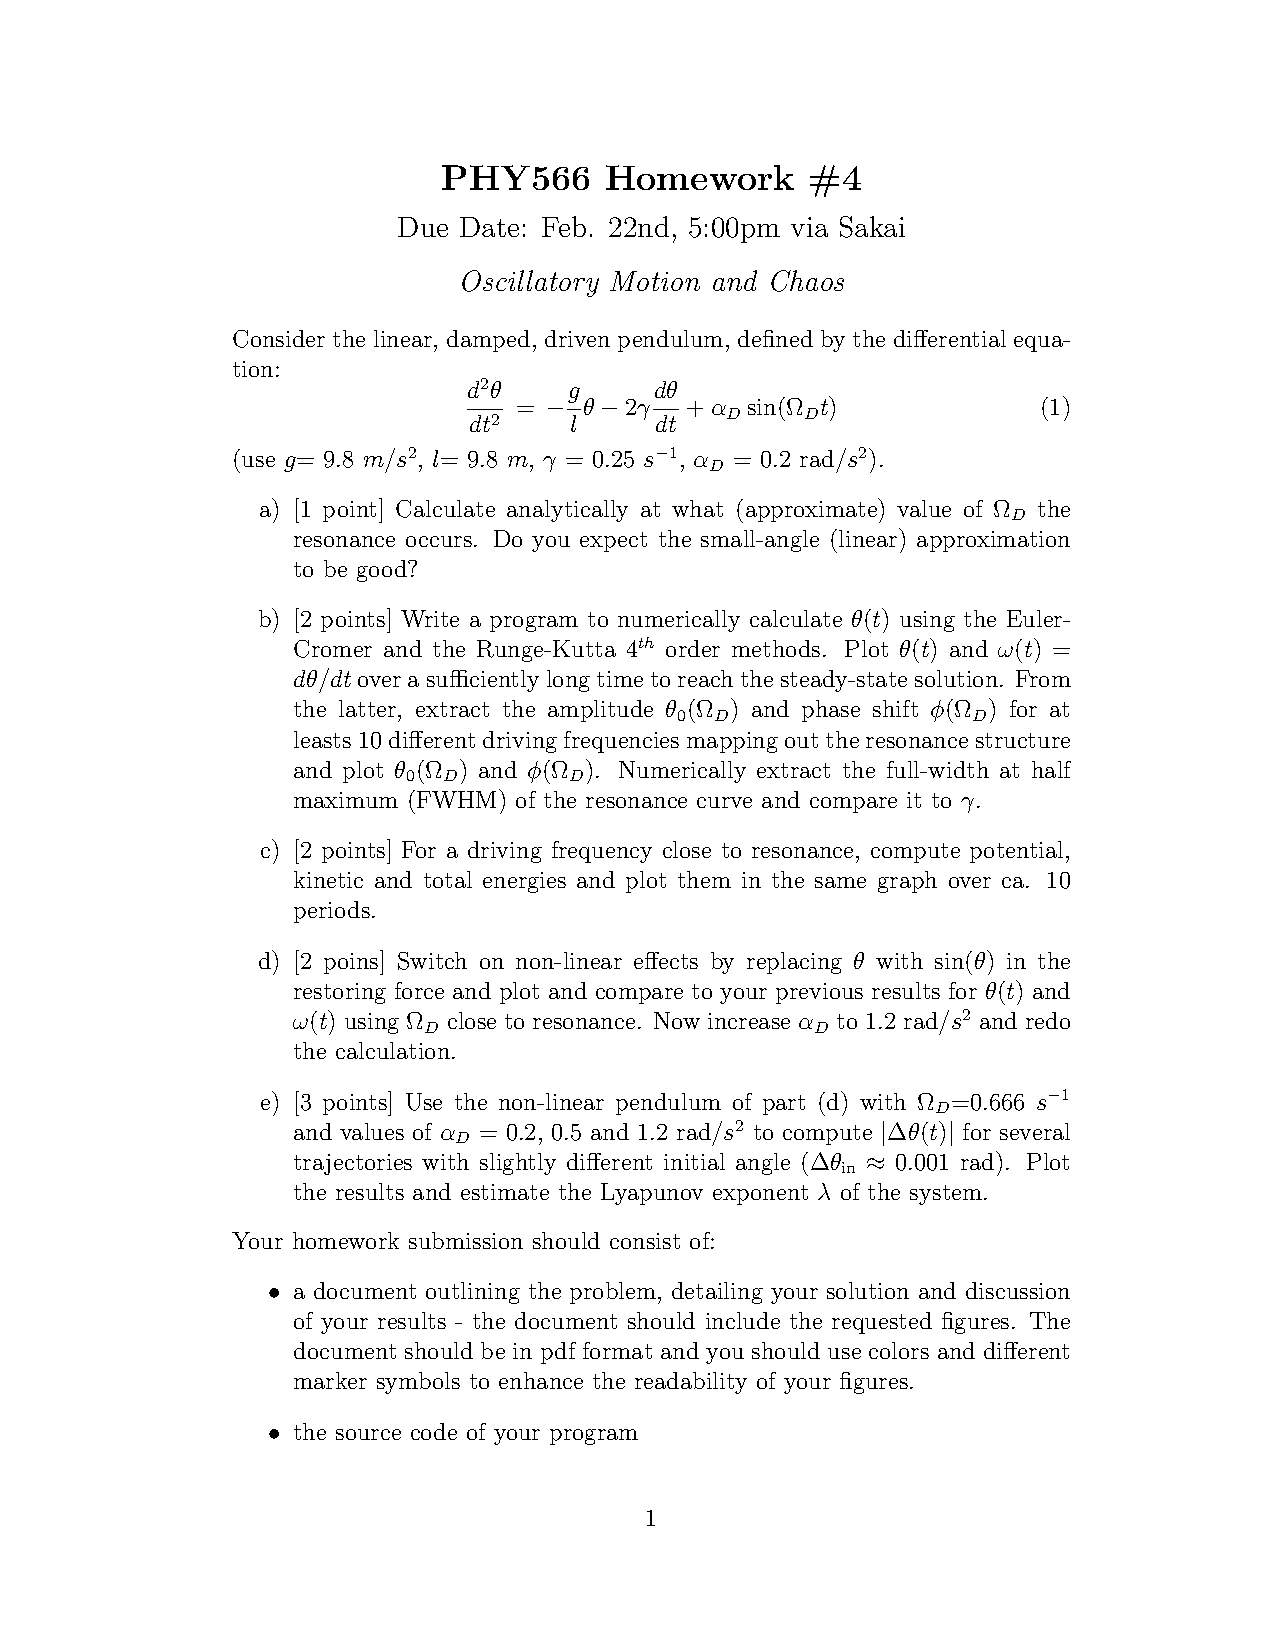
\includepdf{../homework4.pdf}

\clearpage
\section{Code}
\label{sec:code}

\lstinputlisting[style=python]{../code/chaotic_pendulum.py}

\end{document} %%% end of doc %%%
%%%%%%%%%%%%%%%%%%%%%%%%%%%%%%%%%%%%%%%%%%%%%%%%%%%%%


\bibliographystyle{bib_files/styles/atlasBibStyleWoTitle}
\bibliography{bib_files/my_bib.bib}


